% !TeX root = thesis.tex

\chapter{Dataset}\label{ch:dataset}
This chapter discusses the dataset created for training and evaluating the uncertainty-aware object localization models.
We will outline the requirements for the dataset based on the problem statement and objectives defined in \cref{ch:introduction}.
Furthermore, we will describe the data collection process, including the setup and annotation methodology.

\section{Setup}\label{ch:dataset_section:setup}
The setup we used is shown in \cref{fig:setup}, where we have an Intel RealSense camera mounted on a pole overlooking a table with a robotic arm.
The the camera's \gls{fov} is a bit wider and longer than the table, but only the part of the table within the black border lines is usable by the robot.

\begin{figure}
    \centering
    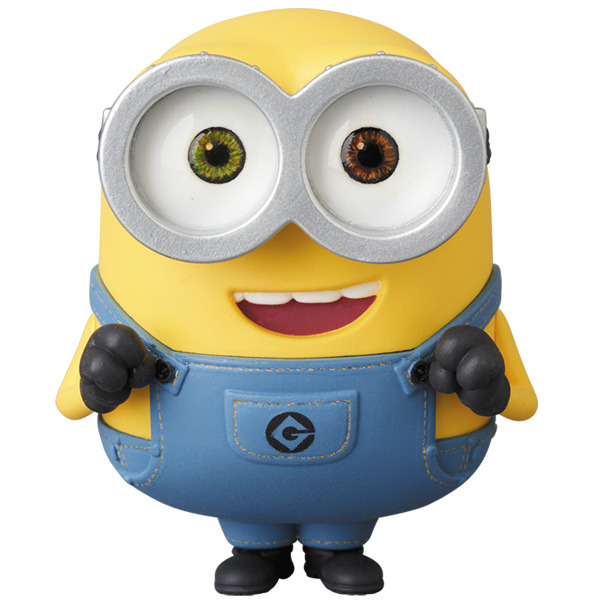
\includegraphics[width=1\textwidth]{static/setup.png}
    \caption{The setup used.}
    \label{fig:setup}
\end{figure}

\subsection{Intel RealSense camera}\label{ch:dataset_section:setup_subsection:realsense-camera}
Intel RealSense cameras are a type of camera which capture both RGB and depth information, the one we used specifically is the ``Intel RealSense Depth Camera D415''.
These cameras have good support in the form of Intel RealSense SDK~\cite{src:RealSense-SDK}.
It is a library which supports different languages like Python, C\#, ROS, etc. and makes it easy to interact with the Intel RealSense cameras.
We will use its Python binding, which is called ``pyrealsense2''.
It allows us to easily set up and handle both the RGB and depth camera streams independently from each other.
It also contains information about the intrinsic parameters of the camera, these embody the focal length and the principal point of the camera.
Its importance will become clear in \cref{ch:dataset_section:labeling_subsection:real-world-coordinates}.

\subsection{Table and robot arm}\label{ch:dataset_section:setup_subsection:table-and-robot-arm}
\paragraph{Table}
The table is used as support for the camera, robot arm and objects.
As \cref{fig:setup} shows, the table is equipped with a grid of black lines in the shape of a rectangle and a black square.
The lines are 2 cm apart from each other and are used as a reference so we can capture the real-world coordinates of the objects.
The black square is used as the origin of this custom coordinate system, more specifically the bottom right corner of the square is the origin.
Relative to the camera's \gls{pov}, the positive x-axis extends horizontally to the right, while the positive y-axis extends vertically downward.
There is no z-axis defined as all the objects are roughly the same height; consequently, the robot arm only needs to know the x and y coordinates of the objects to be able to grasp them.
More information about the specific use of the grid will be given in \cref{ch:dataset_section:labeling_subsection:real-world-coordinates}.

\paragraph{Robot arm}
The robot arm used in our setup is the ``ABB IRB 1200''~\cite{src:ABB-IRB1200}.
It is equipped with a vacuum gripper, which is used to grasp the objects on the table.
The robot arm is controlled by a computer, which sends commands to the robot arm to move to specific coordinates and to open and close the gripper.
Previous work with this specific robot arm~\cite{src:robot-demonstrator} will be used to control it.

\section{Labeling}\label{ch:dataset_section:labeling}
We needed to create a dataset for regression of the position of the objects on the table.
There were three approaches we could take to do this:
\begin{itemize}
    \item We could use the pixel coordinates. 
    \item We could use the real-world coordinates.
    \item We could use the robot's position.
\end{itemize}
There are some advantages and problems with all three approaches.

\subsection{Pixel coordinates}\label{ch:dataset_section:labeling_subsection:pixel-coordinates}
Pixel coordinates are coordinates in the image plane of the camera, they are defined by the number of pixels in the x and y direction.
A computer sees an image as a 2D array of pixels per color channel, so for RGB images, there are 3 2D arrays in total, one for each color channel.
Conventionally, the origin of the pixel coordinates is the first value in the array ($img_r[0][0]$), the x-axis goes horizontally to the right and the y-axis goes vertically downwards.
The libraries most commonly used for computer vision, like OpenCV~\cite{src:open-cv} and PyTorch~\cite{src:pytorch}, use pixel coordinates for their operations on images, which makes it very convenient to use and incorporate.
It makes it easy to annotate the dataset, as we can create a simple script to click on the objects in the images and save the pixel coordinates of the clicks as annotations, as shown in \cref{fig:pixel-annotations}.
Even more, using some of the tools provided by the OpenCV~\cite{src:open-cv} library, we can even automate this clicking process.
Its resulting annotation should be more accurate and consistent than a user clicking on the center of the object, purely visually.
However, it is not 100\% consistent, as some objects were not detected and thus still required some manual clicking.

\begin{figure}
    \centering
    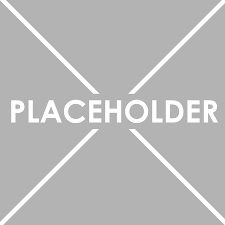
\includegraphics[width=0.8\textwidth]{static/pixel-annotations.png}
    \caption{Annotating the pixel coordinates of the objects.}
    \label{fig:pixel-annotations}
\end{figure}

This way of annotating in pixel space requires some post-processing to achieve what we want, which is the real-world coordinates of the object so the robot arm can use them to grasp the objects.
This transformation requires information about the characteristics of the camera, called the intrinsic parameters, as well as the position and orientation of the camera relative to the table, which are called the extrinsic parameters.
The intrinsic parameters of the camera we are using, are provided by the RealSense SDK~\cite{src:RealSense-SDK} and should be very accurate, as they are measured and provided by the manufacturer.
The extrinsic parameters need to be calibrated for each specific setup, they consist of a rotation and translation from the camera's coordinate system (pixel coordinates) to the table's coordinate system.
OpenCV~\cite{src:open-cv} provides a convenient way to do this calibration, this being the ``findChessboardCorners'' and ``solvePnP'' functions.
It detects the corners of a chessboard pattern, as shown in \cref{fig:cv2-chessboard}, and uses them to calculate the rotation and translation vector using the ``solvePnP'' function.
Once the parameters are obtained, we can use them to transform the pixel coordinates of the objects to real-world coordinates.
However, this process is not perfect and can introduce some errors, which can be a source of uncertainty in the dataset, which is something we want to avoid as much as possible.

\begin{figure}
    \centering
    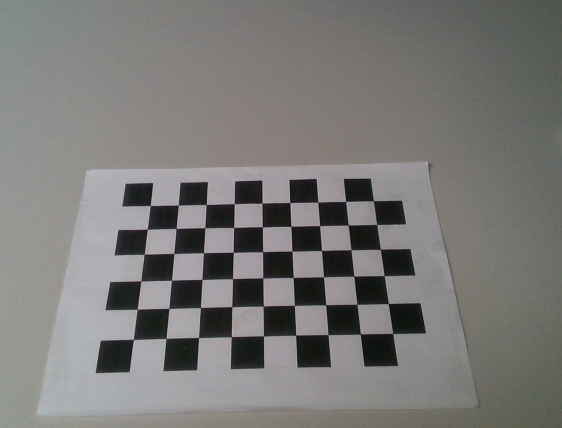
\includegraphics[width=0.8\textwidth]{static/cv2-chessboard.png}
    \caption{The chessboard pattern used for calibration.}
    \label{fig:cv2-chessboard}
\end{figure}

After the translation from pixel coordinates to real-world coordinates, we would need to do another translation from the real-world coordinates to the robot's coordinate system, which is the one used to control the robot arm.
This is a simple translation, as the robot's coordinate system is defined relative to the table's coordinate system.
However, this is yet another step where errors can be introduced, which can again introduce uncertainty in the dataset.

\subsection{Real-world coordinates}\label{ch:dataset_section:labeling_subsection:real-world-coordinates}
We presume real-world coordinates as the coordinates measured in the physical world, in our case they are relative to an origin defined on the table.
Since this way of doing the coordinates uses real measurements, it is more intuitive and directly usable for the robot arm.
However, it comes with an important caveat, as it is more difficult to annotate data efficiently.
We need to define an origin for the coordinate system, as well as the x and y axes, and then we need to measure the coordinates of the objects relative to this origin.
This measuring can be done with a ruler, but this will be too time-consuming and cause too much human error, which can introduce uncertainty in the dataset.
A better option is to use a predefined grid on the table, which we could detect and use to measure the coordinates of the objects.
This is better, as it takes less time to annotate, but we cannot draw a grid on the table, as we would like the \gls{ai} to do inference without any outside assistance (like a grid).
We thus need a way to create a ``virtual'' grid which can easily be removed from the images, but can still be used to measure the coordinates of the objects.
This is where the black lines around the table come in.

They can be detected by the camera~\cite{src:stackoverflow-linedetection} with the help of the OpenCV~\cite{src:open-cv} library and used to create this virtual grid by connecting opposite lines.
\cref{fig:grid} shows what this would look like.
The top and bottom lines are connected (green lines) to create consistent ticks on the x-axis, and the left and right lines are connected (yellow lines) to create consistent ticks on the y-axis.
Since we know the distance between the lines (2 cm), we can use this grid to measure the approximate real-world coordinates of the objects.
For example, the object in \cref{fig:grid} is located in the cell defined by the green and yellow lines 3 and 4, so it is located between 4 and 6 cm on the x- and y-axes.
To reduce the error, and thus uncertainty, linear interpolation can be used within the grid cells to get more accurate coordinates of the objects.
After the annotation process, the image can be cropped to the red box, which removes any evidence of the grid in the images.

\begin{figure}
    \centering
    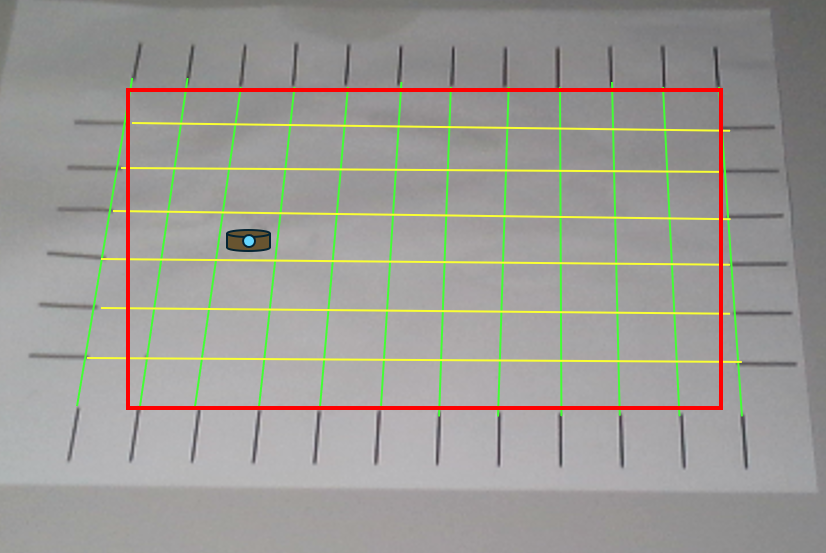
\includegraphics[width=0.8\textwidth]{static/grid.png}
    \caption{The virtual grid created by connecting the opposite lines.}
    \label{fig:grid}
\end{figure}

However, this did not work well, as not all the lines were detected.
This is most probably due to the lighting not being consistent enough for the filters used to detect the lines to work properly.
Another problem is the resolution of the camera being too low to detect the individual lines; this was most prominent in the corners of the table where the lines are closest to each other.

We ended up using a more manual approach, where we manually annotated the pixel coordinates of the center of the lines as well as the origin square.
After this, we could use the same logic as described above to create the virtual grid and measure the real-world coordinates of the objects.
This more manual approach introduces some human error, but still ensured we got a consistent and accurate enough grid.

Now we have a way to measure the real-world coordinates of the objects without introducing too much human error, while still being able to remove the grid from the images so the \gls{ai} can do inference without any outside assistance.
The translation to the robot's coordinate system is however still needed.

\subsection{Robot's position}\label{ch:dataset_section:labeling_subsection:robots-position}
Ultimately, the robot arm needs to move itself to the correct position to be able to grasp the objects.
This means that we could also use the robot's position as labels for the dataset.
However, this, just as the real-world coordinates, is not that easy to annotate, as we need to move the robot arm to the correct position and then read out its coordinates.
There is no easy trick (like using OpenCV~\cite{src:open-cv} for real-world coordinates) to do this fast, accurately but most of all consistent.
We thus would need to manually move the robot to the correct location for each data point.
This would, however, be the way to get the least amount of uncertainty in the dataset by translations, as we would be directly measuring the coordinates that the robot arm needs to move to.
It would be feasible to do this for a set number of robot positions~\cite{src:mp-robot}, and then use interpolation to get the coordinates for the other data points, but this would introduce a lot of error.

This approach takes a lot of time, introduces human error, and lacks consistency; therefore, we opted against using the robot's position as labels for the dataset.

\section{Capturing and using data}\label{ch:dataset_section:capturing-and-saving-data}

\subsection{Collecting data}\label{ch:dataset_section:capturing-and-saving-data_subsection:collecting-data}
To actually capture the data, we created a script which implements both the pixel-coordinate and real-world coordinate approaches, so we can choose which one to ultimately use for our models.
It is an interactive script, which shows the RGB and depth images from the camera in real-time and allows us to capture the data by pressing a button.
When the button is pressed, the script tries to automatically detect the center of the object.
The user can then either accept the detected coordinates or manually click on the center of the object to correct the coordinates.
After pinpointing the object's center, the script crops the image so the calibration lines are not visible anymore and saves the RGB and depth images.
Following this, it calculates the real-world coordinates of the object and saves them alongside the pixel coordinates in a JSON file, which is structured as shown in~\cref{lst:json-structure}.

\begin{listing}
\begin{minted}{json}
{
    "pixel": {
        "x": 221,
        "y": 62
    },
    "world": {
        "x": 288.09246369430474,
        "y": 134.27617670846834
    }
}
\end{minted}
\caption{Example of the JSON file structure.}
\label{lst:json-structure}
\end{listing}

Each trio of RGB image, depth image and JSON file is considered one data point in the dataset, all with a unique identifier.

\subsection{PyTorch Dataset}\label{ch:dataset_section:capturing-and-saving-data_subsection:pytorch-dataset}
Since we are using the PyTorch~\cite{src:pytorch} framework for the training and evaluation of our models, we needed a way to easily load and preprocess the data in a way that is compatible with it.
PyTorch~\cite{src:pytorch} provides a \texttt{Dataset} class, which is an abstract class that we can inherit from and implement our own dataset.

We kept two options open when creating this class, as we wanted to keep as many options open as possible to differentiate between the different approaches.

\begin{itemize}
    \item Have a 3D tensor as input, which is the RGB image, or have a 4D tensor as input, which is the RGB image concatenated with the depth image.
    \item Use the pixel coordinates as labels, or use the real-world coordinates as labels.
\end{itemize}

When looking at the depth images (of which an example is shown in~\cref{fig:sample}) captured by the Realsense camera, we noticed that they did not contain that much information about the object, as the objects are pretty small in height.

\begin{figure}
    \centering
    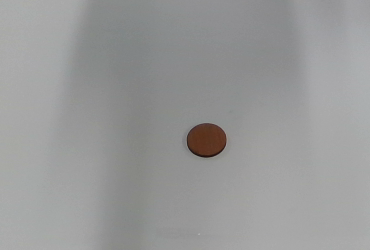
\includegraphics[width=0.49\textwidth]{static/RGB-image.png}
    
\includegraphics[width=0.49\textwidth]{static/depth-image.png}
    \caption{An example of an RGB image with its corresponding depth image captured by the RealSense camera.}
    \label{fig:sample}
\end{figure}

\subsection{Data split}\label{ch:dataset_section:capturing-and-saving-data_subsection:data-split}
We collected a total of 400 data points, all in the same setup, environment and with a single consistent object on the image.
Now that we have the data required, we need to split it into a training and validation set.
These need to stay independent from each other, as we want to evaluate the model's performance on data it has never seen before.
We also wanted to keep a seperate test set, which is used to compare the different models on data similar to the training data, but which is still independent from the training and validation sets.
A common split is 80\% for training, 10\% for validation and 10\% for testing, so this is what we ended up using as well.